\documentclass[a4paper,12pt, twoside]{article}

\textwidth 17cm \textheight 25cm \evensidemargin 0cm
\oddsidemargin 0cm \topmargin -2cm
\parindent 0pt
%\parskip \bigskipamount

\usepackage{graphicx}
\usepackage[dutch]{babel}
\usepackage{amssymb,amsthm,amsmath}
%\usepackage{dot2texi}
\usepackage[utf8]{inputenc}
\usepackage{nopageno}
\usepackage{pdfpages}
\usepackage{enumerate}
\usepackage{caption}
\usepackage{wrapfig}
\usepackage{pgf,tikz,pgfplots}
\pgfplotsset{compat=1.15}
\usepackage{color}
\usetikzlibrary{arrows}
\usetikzlibrary{patterns}
\usepackage{fancyhdr}
\pagestyle{fancy}
\usepackage[version=3]{mhchem}
\usepackage{multicol}
\usepackage{fix-cm}
\usepackage{setspace}
\usepackage{mhchem}
\usepackage{xhfill}
\usepackage{parskip}
\usepackage{cancel}
\usepackage{mdframed}
\usepackage{url}
\usepackage{mathtools}
\usepackage{changepage}

\newcommand{\todo}[1]{{\color{red} TODO: #1}}

\newcommand{\degree}{\ensuremath{^\circ}}
\newcommand\rad{\qopname\relax o{\mathrm{rad}}}

\newcommand\ggd{\qopname\relax o{\mathrm{ggd}}}

\pgfmathdeclarefunction{gauss}{2}{%
  \pgfmathparse{1/(#2*sqrt(2*pi))*exp(-((x-#1)^2)/(2*#2^2))}%
}

\def\LRA{\Leftrightarrow}

\newcommand{\zrmbox}{\framebox{\phantom{EXE}}\phantom{X}}
\newcommand{\zrm}[1]{\framebox{#1}}

% environment oefening:
% houdt een teller bij die de oefeningen nummert, probeert ook de oefening op één pagina te houden
\newcounter{noefening}
\setcounter{noefening}{0}
\newenvironment{oefening}
{
  \stepcounter{noefening}
  \pagebreak[0]
  \begin{minipage}{\textwidth}
  \vspace*{0.7cm}{\large\bf Oefening \arabic{noefening}}
}{%
  \end{minipage}
}

\usepackage{calc}

% vraag
\reversemarginpar
\newcounter{punten}
\setcounter{punten}{0}
\newcounter{nvraag}
\setcounter{nvraag}{1}
\newlength{\puntwidth}
\newlength{\boxwidth}
\newcommand{\vraag}[1]{
\settowidth{\puntwidth}{\Large{#1}}
\setlength{\boxwidth}{1.5cm}
\addtolength{\boxwidth}{-\puntwidth}
{\large\bf Vraag \arabic{nvraag} \addtocounter{nvraag}{1}}\vspace*{-0.5cm}
{\marginpar{\color{lightgray}\fbox{\parbox{1.5cm}{\vspace*{1cm}\hspace*{\boxwidth}{\Large{#1}}}}}
\vspace*{0.5cm}}
\addtocounter{punten}{#1}}

% arulefill
\def\arulefill{\leavevmode{\xrfill[-5pt]{0.3pt}[lightgray]\endgraf}\vspace*{0.2cm}}

% \arules{n}
\newcommand{\arules}[1]{
\color{lightgray}
%\vspace*{0.05cm}
\foreach \n in {1,...,#1}{
  \vspace*{0.75cm}
  \hrule height 0.3pt\hfill
}\color{black}\vspace*{0.2cm}}

% \arule{x}
\newcommand{\arule}[1]{
\color{lightgray}{\raisebox{-0.1cm}{\rule[-0.05cm]{#1}{0.3pt}}}\color{black}
}

% \abox{y}
\newcommand{\abox}[1]{
\fbox{
\begin{minipage}{\textwidth- 4\fboxsep}
\hspace*{\textwidth}\vspace{#1}
\end{minipage}
}
}

\newcommand{\ruitjes}[1]{
\definecolor{cqcqcq}{rgb}{0.85,0.85,0.85}
\hspace*{-2.5cm}
\begin{tikzpicture}[scale=1.04,line cap=round,line join=round,>=triangle 45,x=1.0cm,y=1.0cm]
\draw [color=cqcqcq, xstep=0.5cm, ystep=0.5cm] (0,-#1) grid (20.5,0);
\end{tikzpicture}
}


\newcommand{\assenstelsel}[5][1]{
\definecolor{cqcqcq}{rgb}{0.65,0.65,0.65}
\begin{tikzpicture}[line cap=round,line join=round,>=triangle 45,x=#1cm,y=#1cm]
\draw [color=cqcqcq,dash pattern=on 1pt off 1pt, xstep=1.0cm,ystep=1.0cm] (#2,#4) grid (#3,#5);
\draw[->,color=black] (#2,0) -- (#3,0);
%\draw[shift={(1,0)},color=black] (0pt,2pt) -- (0pt,-2pt) node[below] {\footnotesize $1$};
%\draw[color=black] (#3.25,0.07) node [anchor=south west] {$x$};
\draw[->,color=black] (0,#4) -- (0,#5);
%\draw[shift={(0,1)},color=black] (2pt,0pt) -- (-2pt,0pt) node[left] {\footnotesize $1$};
\draw[color=black] (0.09,#5.25) node [anchor=west] {\phantom{$y$}};
%\draw[color=black] (0pt,-10pt) node[right] {\footnotesize $0$};
\end{tikzpicture}
}

\newcommand{\getallenas}[3][1]{
\definecolor{cqcqcq}{rgb}{0.65,0.65,0.65}
\begin{tikzpicture}[scale=#1,line cap=round,line join=round,>=triangle 45,x=1.0cm,y=1.0cm]
\draw [color=cqcqcq,dash pattern=on 1pt off 1pt, xstep=1.0cm,ystep=1.0cm] (#2,-0.2) grid (#3,0.2);
\draw[->,color=black] (#2.25,0) -- (#3.5,0);
\draw[shift={(0,0)},color=black] (0pt,2pt) -- (0pt,-2pt) node[below] {\footnotesize $0$};
\draw[shift={(1,0)},color=black] (0pt,2pt) -- (0pt,-2pt) node[below] {\footnotesize $1$};
\draw[color=black] (#3.25,0.07) node [anchor=south west] {$\mathbb{R}$};
\end{tikzpicture}
}

\newcommand{\visgraad}[1]{\begin{tabular}{p{0.5cm}|p{#1}}&\\\hline\\\end{tabular}}

\newcommand{\tekenschema}[2]{\begin{tabular}{p{0.5cm}|p{#1}}&\\\hline\\[#2]\end{tabular}}

% schema van Horner
\newcommand{\schemahorner}{
\begin{tabular}{p{0.5cm}|p{7cm}}
&\\[1.5cm]
\hline\\
\end{tabular}}

% geef tabular iets meer ruimte
\setlength{\tabcolsep}{14pt}
\renewcommand{\arraystretch}{1.5}

\newcommand{\toets}[3]{
\thispagestyle{plain}
\vspace*{-2.5cm}
\begin{tikzpicture}[remember picture, overlay]
    \node [shift={(15.25 cm,-1.6cm)}] {%
        \includegraphics[width=1.8cm]{/home/ppareit/kaa1415/logokaavelgem.png}%
    };%
\end{tikzpicture}

\begin{tabular}{|llc|c|}
\hline
\vspace*{-0.5cm}
&&&\\
Naam & \arule{4cm} & {\Large\bf KA AVELGEM} & \\
\vspace*{-0.75cm}
&&&\\
Klas & \arule{4cm} & {\Large\bf 20...-...-...} & \\
\hline
\vspace*{-0.75cm}
&&&\\
Toets & {\bf #2} & {\large\bf #1} & Beoordeling\\
\vspace*{-0.75cm}
&&&\\
Onderwerp & \multicolumn{2}{l|}{\bf #3} &\\
\hline
\end{tabular}
}

\newcommand{\oefeningen}[1]{

\fancyhead[LE, RO]{\vspace{0.5cm} #1}
%\thispagestyle{plain}

{\bf \Large \centering Oefeningen: #1}

}

\raggedbottom

\newcommand\vl{\qopname\relax o{\mathrm{vl}}}

\newcommand\dom{\qopname\relax o{\mathrm{dom}}}
\newcommand\ber{\qopname\relax o{\mathrm{ber}}}

\newcommand\mC{\qopname\relax o{\mathrm{mC}}}
\newcommand\uC{\qopname\relax o{\mathrm{{\mu}C}}}
\newcommand\C{\qopname\relax o{\mathrm{C}}}

\newcommand\W{\qopname\relax o{\mathrm{W}}}
\newcommand\kW{\qopname\relax o{\mathrm{kW}}}
\newcommand\kWh{\qopname\relax o{\mathrm{kWh}}}


\newcommand\V{\qopname\relax o{\mathrm{V}}}
\newcommand\ohm{\qopname\relax o{\mathrm{\Omega}}}
\newcommand\kohm{\qopname\relax o{\mathrm{k\Omega}}}


\newcommand\N{\qopname\relax o{\mathrm{N}}}

\newcommand\Nperkg{\qopname\relax o{\mathrm{N/kg}}}

\newcommand\Nperm{\qopname\relax o{\mathrm{N/m}}}

\newcommand\gpermol{\qopname\relax o{\mathrm{g/mol}}}


\newcommand\kgperm{\qopname\relax o{\mathrm{kg/m}}}
\newcommand\kgperdm{\qopname\relax o{\mathrm{kg/dm}}}
\newcommand\gpercm{\qopname\relax o{\mathrm{g/cm}}}
\newcommand\gperml{\qopname\relax o{\mathrm{g/ml}}}


\newcommand{\mA}{\;\mbox{mA}}
\newcommand{\A}{\;\mbox{A}}
\newcommand{\MA}{\;\mbox{MA}}

\newcommand{\us}{\;\mu\mbox{s}}
\newcommand\s{\qopname\relax o{\mathrm{s}}}

\newcommand\h{\qopname\relax o{\mathrm{h}}}

\newcommand{\kmperh}{\;\mbox{km/h}}
\newcommand{\mpers}{\;\mbox{m/s}}
\newcommand{\kmpermin}{\;\mbox{km/min}}
\newcommand{\kmpers}{\;\mbox{km/s}}

\newcommand{\mph}{\;\mbox{mph}}

\newcommand{\Hz}{\;\mbox{Hz}}

\newcommand\Gm{\qopname\relax o{\mathrm{Gm}}}
\newcommand\Mm{\qopname\relax o{\mathrm{Mm}}}
\newcommand\km{\qopname\relax o{\mathrm{km}}}
\newcommand\hm{\qopname\relax o{\mathrm{hm}}}
\newcommand\dam{\qopname\relax o{\mathrm{dam}}}
\newcommand\m{\qopname\relax o{\mathrm{m}}}
\newcommand\dm{\qopname\relax o{\mathrm{dm}}}
\newcommand\cm{\qopname\relax o{\mathrm{cm}}}
\newcommand\mm{\qopname\relax o{\mathrm{mm}}}
\newcommand\um{\qopname\relax o{\mathrm{{\mu}m}}}
\newcommand\nm{\qopname\relax o{\mathrm{nm}}}


\newcommand\Gg{\qopname\relax o{\mathrm{Gg}}}
\newcommand\Mg{\qopname\relax o{\mathrm{Mg}}}
\newcommand\kg{\qopname\relax o{\mathrm{kg}}}
\newcommand\hg{\qopname\relax o{\mathrm{hg}}}
\renewcommand\dag{\qopname\relax o{\mathrm{dag}}}
\newcommand\g{\qopname\relax o{\mathrm{g}}}
\newcommand\dg{\qopname\relax o{\mathrm{dg}}}
\newcommand\cg{\qopname\relax o{\mathrm{cg}}}
\newcommand\mg{\qopname\relax o{\mathrm{mg}}}
\newcommand\ug{\qopname\relax o{\mathrm{{\mu}g}}}
\renewcommand\ng{\qopname\relax o{\mathrm{ng}}}

\newcommand\ton{\qopname\relax o{\mathrm{ton}}}

\newcommand\Gl{\qopname\relax o{\mathrm{Gl}}}
\newcommand\Ml{\qopname\relax o{\mathrm{Ml}}}
\newcommand\kl{\qopname\relax o{\mathrm{kl}}}
\newcommand\hl{\qopname\relax o{\mathrm{hl}}}
\newcommand\dal{\qopname\relax o{\mathrm{dal}}}
\renewcommand\l{\qopname\relax o{\mathrm{l}}}
\newcommand\dl{\qopname\relax o{\mathrm{dl}}}
\newcommand\cl{\qopname\relax o{\mathrm{cl}}}
\newcommand\ml{\qopname\relax o{\mathrm{ml}}}
\newcommand\ul{\qopname\relax o{\mathrm{{\mu}l}}}
\newcommand\nl{\qopname\relax o{\mathrm{nl}}}

\newcommand\MJ{\qopname\relax o{\mathrm{MJ}}}
\newcommand\kJ{\qopname\relax o{\mathrm{kJ}}}
\newcommand\J{\qopname\relax o{\mathrm{J}}}

\newcommand\T{\qopname\relax o{\mathrm{T}}}
\newcommand\uT{\qopname\relax o{\mathrm{{\mu}T}}}

\newcommand\grC{\qopname\relax o{\mathrm{{\degree}C}}}

\newcommand\K{\qopname\relax o{\mathrm{K}}}
\newcommand\calperK{\qopname\relax o{\mathrm{cal/K}}}

\newcommand\hPa{\qopname\relax o{\mathrm{hPa}}}
\newcommand\Pa{\qopname\relax o{\mathrm{Pa}}}

\newcommand\dB{\qopname\relax o{\mathrm{dB}}}

\newcommand\Var{\qopname\relax o{\mathrm{Var}}}

\newcommand{\EE}[1]{\cdot 10^{#1}}

\onehalfspacing

%\setlength{\headsep}{0cm}

\newenvironment{exlist}[1] %
{ \begin{multicols}{#1}
  \begin{enumerate}[(a)]
    \setlength{\itemsep}{0.5em} }
{ \end{enumerate}
  \end{multicols} }




\begin{document}

\begin{center}
  \begin{mdframed}
  \centering
  \fontsize{40}{50}\selectfont Integraalrekening
  \end{mdframed}
  \vfill
  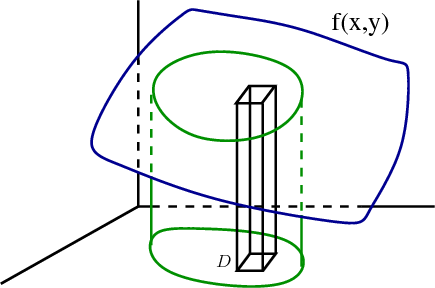
\includegraphics[width=.5\textwidth]{double_integral_volume_under_surface_box}
  \vfill
\end{center}

\begin{singlespacing}
\subsection*{Doelstelling}
\small
Je \hfill  {\scriptsize(LP 2006-059, LI 1.10)}
\begin{itemize}
  \item kan het begrip differentiaal en de meetkundige betekenis ervan
  \item kent het begrip bepaalde integraal
  \item kan het verband uitleggen tussen de bepaalde integraal van een functie en de oppervlakte van een gebied bepaald door de functie en de $x$-as
  \item kent het begrip primitieve functie
  \item kent de onderstaande eigenschappen:
  \begin{itemize}
    \item de stelling in verband met de optelbaarheid van de bepaalde integraal,
    \item de middelwaardenstelling,
    \item de hoofdstelling van de integraalrekening,
    \item de stelling in verband met de lineariteit van de bepaalde integraal,
    \item de stelling in verband met de bepaalde integraal en ongelijkheden
  \end{itemize}
  \item kan het verband illustreren tussen het berekenen van de bepaalde integraal van een functie en de primitieve van de gegeven functie
  \item kan bij het integreren van eenvoudige veeltermfuncties, rationale functies, irrationale functies, exponentiële functies, logaritmische functies en goniometrische functies gebruik maken van:
  \begin{itemize}
    \item de basisformules van de integraalrekening;
    \item de substitutiemethode;
    \item de methode van partiële integratie
  \end{itemize}
  \item kan vraagstukken/problemen oplossen (ook van buiten de wiskunde) die kunnen herleid worden tot het berekenen van een integraal
\end{itemize}
\end{singlespacing}

\thispagestyle{empty}
\newpage

\tableofcontents
\thispagestyle{empty}
\newpage

\pagenumbering{arabic}

\pagestyle{fancy}
\fancyhead[RO,LE]{Integraalrekening}
\fancyhead[RE,LO]{}

\cleardoublepage
\section{Differentiaal}

\subsection{Differentiaal van een willekeurige functie}

In volgende figuur kennen we het verloop van de functie $f$ tot aan $x=a$. We willen een voorspelling doen over $f(b)$. Noem $\Delta x=b-a$. We willen dus weten wat $\Delta y=f(b)-f(a)$ is. We zijn tevreden met een benadering van $\Delta y$.

\begin{center}
\definecolor{wqwqwq}{rgb}{0.38,0.38,0.38}
\definecolor{uququq}{rgb}{0.25,0.25,0.25}
\begin{tikzpicture}[scale=1.1,line cap=round,line join=round,>=triangle 45,x=1.0cm,y=1.0cm]
\draw[->,color=black] (-3.3,0) -- (7.19,0);
\foreach \x in {-2,2,4,6}
\draw[shift={(\x,0)},color=black] (0pt,2pt) -- (0pt,-2pt);
\draw[->,color=black] (0,-1.41) -- (0,4.84);
\foreach \y in {,2,4}
\draw[shift={(0,\y)},color=black] (2pt,0pt) -- (-2pt,0pt);
\clip(-3.3,-1.41) rectangle (7.19,4.84);
\draw(2.93,6.98) -- (5.18,6.98);
\draw[line width=1.6pt, smooth,samples=100,domain=-3.302227053746148:7.191102772295233] plot(\x,{1/500*((\x)+2.5)*((\x)-6.5)*((\x)+0.5)*((\x)-3.5)*((\x)-9.5)+3});
\draw(2.88,7.93) -- (5.14,7.93);
\draw [line width=1.2pt,dotted,color=wqwqwq,domain=-3.3:7.19] plot(\x,{(--0.95--0.46*\x)/1});
\draw (-2.78,3.55) node[anchor=north west] {f};
\draw (2,1.86)-- (4,1.86);
\draw (4,1.86)-- (4,3.4);
\draw (2.81,1.86) node[anchor=north west] {$\Delta x$};
\begin{scriptsize}
\fill [color=black] (4.05,6.98) circle (1.5pt);
\draw[color=black] (4.19,7.39) node {$b = 4$};
\fill [color=black] (4.01,7.93) circle (1.5pt);
\draw[color=black] (4.14,8.34) node {$a = 2$};
\fill [color=uququq] (4,1.86) circle (1.5pt);
\draw[color=uququq] (4.23,1.64) node {$C$};
\draw[color=wqwqwq] (-2.67,-0.55) node {$t$};
\fill [color=uququq] (2,1.86) circle (1.5pt);
\draw[color=uququq] (1.68,2.31) node {$A$};
\fill [color=uququq] (4,3.4) circle (1.5pt);
\draw[color=uququq] (3.92,3.87) node {$B$};
\fill [color=uququq] (4,2.77) circle (1.5pt);
\draw[color=uququq] (4.33,2.65) node {$D$};
\fill [color=uququq] (2,0) circle (1.5pt);
\draw[color=uququq] (2.02,-0.35) node {a};
\fill [color=uququq] (4,0) circle (1.5pt);
\draw[color=uququq] (4.03,-0.35) node {b};
\end{scriptsize}
\end{tikzpicture}
\end{center}

Voor de eenvoud noemen we $(a,f(a))=A$, $(b,f(b))=B$ en $(b,f(a))=C$. We zoeken dus de afstand $\Delta y=|BC|$. Teken nu de raaklijn $t$ van $f$ in $A$ en noem het snijpunt $BC \cap t=D$. Als $A$ en $B$ voldoende dicht bij elkaar liggen wordt $\Delta y$ benaderd door $|CD|$.

We berekenen nu de rico $m$ van $t$ op 2 manieren:
\begin{itemize}
\item M.b.v. definitie rico waarbij $(x_1,y_1)$ en $(x_2, y_2)$ zelf te kiezen punten op $t$ zijn:
  $$m=\dfrac{y_2-y_1}{x_2-x_1}=\dfrac{y_D-y_A}{x_D-x_A}=\dfrac{y_D-y_C}{b-a}=\dfrac{y_D-y_C}{\Delta x}$$
\item M.b.v. afgeleide waarde van $f$ in $a$. We kunnen kiezen om deze te berekenen in $a$ omdat de raaklijn $t$ een rechte is en dus zal de afgeleide waarde overal dezelfde zijn.
  $$m = f'(a)$$
\end{itemize}

Onze rico elimineren we uit bovenstaande vergelijkingen:
\begin{align*}
     f'(a)       & = \dfrac{y_D-y_C}{\Delta x}                \\
\lra \qquad y_D - y_C & = f'(a)\cdot \Delta x                          \\
                 & = \mbox{differentiaal van $f$ in $a$} \\
                 & = \mbox{benadering voor $\Delta y$}        \\
\end{align*}

We noteren deze benadering als $df(a)$. Merk op dat we uit de notatie de afstand $\Delta x$ laten verdwijnen. Dit omdat we in de toekomst $\Delta x$ oneindig klein zullen veronderstellen. Zodoende wordt de benadering exact! We krijgen dus volgende definitie.

\subsection{Definitie}
Voor een functie $f$ die afleidbaar is in $x$ en voor een $\Delta x$ die een toename is die oneindig klein wordt noemen we de differentiaal van $f$ in $x$ het product
$$df(x)=f'(x)\cdot\Delta x$$

\begin{oefening}
Bereken
\begin{multicols}{2}
\begin{enumerate}[(a)]
  \itemsep1em
  \item $\displaystyle d(x^4)$
  \item $\displaystyle d(\ln x)$
  \item $\displaystyle d(\sin x)$
  \item $\displaystyle d(x^3-2x)$
\end{enumerate}
\end{multicols}
\end{oefening}

\subsection{Elimineren van $\Delta x$}

We berekenen de differentiaal van $f(x)=x$:
\begin{align*}
  df(x) &= f'(x)\Delta x\\
        &= x' \Delta x\\
        &= 1 \Delta x\\
        &= \Delta x\\
\end{align*}
Maar $df(x) = dx$ en dus $\Delta x = dx$. We mogen onze definitie dus aanpassen tot
$$df(x)=f'(x)\cdot dx$$

\begin{oefening}
Bereken
\begin{multicols}{2}
\begin{enumerate}[(a)]
  \itemsep1em
  \item $\displaystyle d\left(\dfrac{1}{x^2}\right)$
  \item $\displaystyle d\left(\log_2 x\right)$
  \item $\displaystyle d\left(\tan x\right)$
  \item $\displaystyle d\left(\frac{1}{3}x^3+\frac{1}{2}x^2+x+1\right)$
\end{enumerate}
\end{multicols}
\end{oefening}

\needspace{4cm}
\subsection{Rekenregels voor het differentiëren}

\begin{mdframed}
\begin{multicols}{2}
  \begin{align*}
    dc &= 0\\
    dx^n &= nx^{n-1}dx\\
    d\sqrt{x}&=\dfrac{1}{2\sqrt{x}}dx\\
  \end{align*}
  \begin{align*}
    d(f+g) &= df + dg\\
    d(f\cdot g) &= df\cdot g + f\cdot dg\\
    d(c\cdot f) &= c\cdot f\\
    d\left(\dfrac{f}{g}\right) &=\dfrac{df\cdot g - f\cdot dg}{g^2}
  \end{align*}
  \begin{align*}
    de^x &= e^xdx\\
    da^x &= a^x\ln(a) dx\\
  \end{align*}
  \begin{align*}
    d\ln(x) &= \dfrac{1}{x}dx\\
    d\log_a(x) &= \dfrac{1}{x\cdot\ln a}dx\\
  \end{align*}
  \begin{align*}
    d\sin x &= \cos x \cdot dx\\
    d\cos x &= -\sin x \cdot dx\\
    d\tan x &= \dfrac{1}{\cos^2 x} \cdot dx\\
  \end{align*}
\end{multicols}
\end{mdframed}

Merk op dat we de kettingregel gratis krijgen! Zie volgende voorbeeld:

\begin{align*}
  d\sin\sqrt{x} &= \cos\sqrt{x} \cdot d\sqrt{x}\\
                &= \cos\sqrt{x} \cdot \dfrac{1}{2\sqrt{x}} \cdot dx\\
                &= \dfrac{\cos\sqrt{x}}{2\sqrt{x}} dx
\end{align*}

\begin{oefening}
Bepaal de differentiaal van de volgende functies
\begin{multicols}{2}
\begin{enumerate}[(a)]
  \itemsep.5em
  \item $\displaystyle f(x)=x^3+x$
  \item $\displaystyle f(x)=(x-2)(x+2)-x^2$
  \item $\displaystyle f(x)=5+3x^2+8x^4$
  \item $\displaystyle f(x)=\left(2x-4\right)^3$
  \item $\displaystyle f(x)=\left(x^2+x^4+x^6\right)^4$
  \item $\displaystyle f(x)=\sqrt{x^2+2x}$
  \item $\displaystyle f(x)=\sqrt[5]{6x^5+5x}$
  \item $\displaystyle f(x)=x^2\cdot\sqrt{x}$
  \item $\displaystyle f(x)=x^2\cdot\sqrt{x+1}$
  \item $\displaystyle f(x)=\dfrac{2x+1}{2x-1}$
  \item $\displaystyle f(x)=\dfrac{x^2-1}{x-1}$
  \item $\displaystyle f(x)=\dfrac{x^2-1}{x^2+1}$
  \item $\displaystyle f(x)=\dfrac{x^3+3x^2+3x+1}{x+1}$
  \item $\displaystyle f(x)=4^{x}$
  \item $\displaystyle f(x)=e^{-2x}$
  \item $\displaystyle f(x)=e^{\sqrt[3]{3x}}$
  \item $\displaystyle f(x)=\log_2 x$
  \item $\displaystyle f(x)=\log_2 (x^2-9)$
  \item $\displaystyle f(x)=x\cdot \ln x$
  \item $\displaystyle f(x)=x\cdot \ln x^2$
  \item $\displaystyle f(x)=\dfrac{1}{\ln 10}\cdot 10^{x^2}$
  \item $\displaystyle f(x)=x\sin x + \cos x$
\end{enumerate}
\end{multicols}
\end{oefening}

\subsection{Toepassing}

Benader de waarde van $\log_2 5$, veronderstel dat je rekentoestel geen logaritmen kan uitrekenen maar dat je wel weet dat $\ln 2 \approx 0.7$ is.

\begin{center}
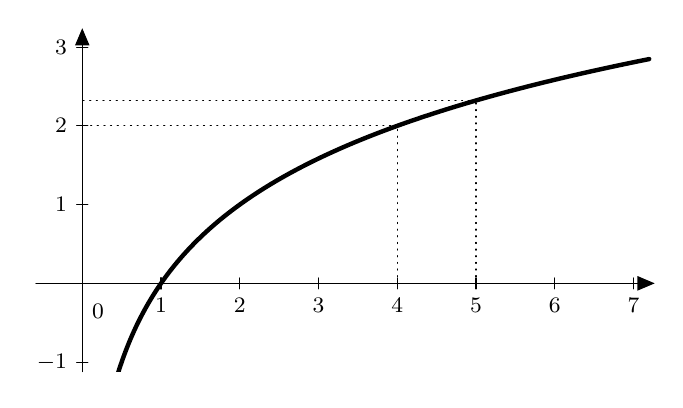
\begin{tikzpicture}[line cap=round,line join=round,>=triangle 45,x=1.0cm,y=1.0cm]
\draw[->,color=black] (-0.59,0) -- (7.27,0);
\foreach \x in {,1,2,3,4,5,6,7}
\draw[shift={(\x,0)},color=black] (0pt,2pt) -- (0pt,-2pt) node[below] {\footnotesize $\x$};
\draw[->,color=black] (0,-1.12) -- (0,3.24);
\foreach \y in {-1,1,2,3}
\draw[shift={(0,\y)},color=black] (2pt,0pt) -- (-2pt,0pt) node[left] {\footnotesize $\y$};
\draw[color=black] (0pt,-10pt) node[right] {\footnotesize $0$};
\clip(-0.59,-1.12) rectangle (7.27,3.24);
\draw[line width=1.6pt, smooth,samples=100,domain=0.1:7.2] plot(\x,{ln((\x))/ln(2)});
\draw [dotted] (4,0)-- (4,2);
\draw [dotted] (5,0)-- (5,2.32);
\draw [dotted] (4,2)-- (0,2);
\draw [dotted] (5,2.32)-- (0,2.32);
\end{tikzpicture}
\end{center}

Stel $f(x)=\log_2(x)$ en neem een waarde $x=4$ dicht bij de waarde $5$ die we willen benaderen.

We berekenen
\begin{enumerate}
  \item $\Delta x = 5-4 = 1$
  \item $\Delta y = \log_2(5) - \log_2(4) = \log_2(5) - 2$
  \item $df(x)=d\log_2(x)=\dfrac{1}{x\ln 2} dx$
\end{enumerate}

We maken nu gebruik van het feit dat $\Delta x=dx$ en $\Delta y \approx dy$ met $dy=df(9)$
\begin{align*}
    &&      \Delta y &\approx df(4)\\
\lra&& \log_2(5) - 2 &\approx \dfrac{1}{4\ln 2} \cdot 1\\
\lra&&     \log_2(5) &\approx 2 + \dfrac{1}{4\ln 2} \cdot 1\\
\lra&&     \log_2(5) &\approx 2 + \dfrac{1}{4\cdot 0.7}\\
\lra&&     \log_2(5) &\approx 2.36\\
\end{align*}

De werkelijke waarde afgerond op 2 decimalen is $\log_2 5 = 2.32$. We hebben dus een fout van 4 honderdsten.

\begin{oefening}
Benader
\begin{multicols}{3}
\begin{enumerate}[(a)]
  \itemsep.5em
  \item $\displaystyle \sqrt[3]{9}$
  \item $\displaystyle \sqrt{24}$
  \item $\displaystyle e^{0.2}$
  \item $\displaystyle \sqrt{9.5}$
  % next are from https://www.math24.net/approximation-differentials/
  \item $\displaystyle \sqrt[3]{30}$
  \item $\displaystyle \sqrt{50}$
  \item $\displaystyle \sqrt[4]{0.025}$
  \item $\displaystyle 8.2^\frac{2}{3}$
\end{enumerate}
\end{multicols}
\end{oefening}

\begin{oefening} % bron http://info.math4all.nl/MathAdore/vb-bb43-ex2b.html
De luchtdruk $p$ (in hectopascal $\hPa$) hangt af van de hoogte $h$ in $\km$ boven het aardoppervlak. In een luchtballon is de luchtdruk gemakkelijk te meten en wordt daaruit de hoogte berekend met de formule:
$$h = -6.5 \log \frac{p}{p_0}$$
Hierin is $p_0$ de luchtdruk op zeeniveau. Neem aan dat $p_0 = 1000 \hPa$.
Bereken nu de hoogte en de snelheid waarmee $h(p)$ verandert als $p = 920 \hPa$ wordt gemeten.
\end{oefening}

\cleardoublepage
\section{Bepaalde integraal}

\subsection{Definitie}

We beschouwen een willekeurige functie $y=f(x)$, positief tussen $a$ en $b$, en berekenen de oppervlakte $S$ begrepen tussen
\begin{itemize}
  \item de $x$-as: $y=0$,
  \item de grafiek van $y=f(x)$,
  \item de verticale $x=a$,
  \item de verticale $x=b$.
\end{itemize}

\begin{center}
\definecolor{dcrutc}{rgb}{0.8627,0.0784,0.2353}
\definecolor{sqsqsq}{rgb}{0.1255,0.1255,0.1255}
\begin{tikzpicture}[scale=1.5,line cap=round,line join=round,>=triangle 45,x=1.0cm,y=1.0cm]
\draw[->,color=black] (-1.3618,0) -- (7.1769,0);
\draw[color=black] (6.9069,0.0675) node [anchor=south west] { x};
\draw[->,color=black] (0,-1.2111) -- (0,3.5477);
\draw[color=black] (0.0844,3.2102) node [anchor=west] { y};
\clip(-1.3618,-1.2111) rectangle (7.1769,3.5477);
\draw[color=sqsqsq,fill=sqsqsq,fill opacity=0.1] {[smooth,samples=50,domain=1.0:6.0] plot(\x,{sin((2*\x-3)*180/pi)-(\x-3)^2/10+2})} -- (6,0) {[smooth,samples=50,domain=6.0:1.0] -- plot(\x,{0})} -- (1,0.7585) -- cycle;
\draw[line width=1.6pt, smooth,samples=100,domain=0.5:6.5] plot(\x,{sin((2*(\x)-3)*180/pi)-((\x)-3)^2/10+2});
\fill [color=black] (1,0) circle (2.0pt);
\draw[color=black] (1,-0.2) node {a};
\fill [color=black] (6,0) circle (2.0pt);
\draw[color=black] (6,-0.2) node {b};
\draw[color=black] (1.4,2.4) node {$f$};
\draw[color=black] (3,1) node {$S$};
\end{tikzpicture}
\end{center}

\begin{itemize}
  \item Verdeel $[a,b]$ in $n$ gelijke deelintervallen, elk met lengte
  $$\Delta x=\dfrac{b-a}{n}$$
  We krijgen dus de $n$ gelijke deelintervallen
  $$[x_0, x_1],[x_1, x_2],\ldots,[x_{n-1}, x_{n}]$$
  \item Het $k$-de interval, namelijk $[x_{k-1},x_{k}]$, heeft een
  \begin{itemize}
    \item kleinste functiewaarde: $\min_k f$
    \item grootste functiewaarde: $\max_k f$
  \end{itemize}
  \item We berekenen voor alle intervallen samen de
  \begin{itemize}
    \item ondersom (som van de oppervlakten rechthoekjes onder de functie),
    \begin{align*}
      s_n &= \min\nolimits_1 f\cdot \Delta x + \min\nolimits_2 f\cdot \Delta x + \ldots + \min\nolimits_n f\cdot \Delta x\\
          &= \sum_{k=1}^n \min\nolimits_k f\cdot\Delta x
    \end{align*}
    \item bovensom (som van de oppervlakten rechthoekjes boven de functie),
    \begin{align*}
      S_n &= \max\nolimits_1 f\cdot \Delta x + \max\nolimits_2 f\cdot \Delta x + \ldots + \max\nolimits_n f\cdot \Delta x\\
          &= \sum_{k=1}^n \max\nolimits_k f\cdot\Delta x
    \end{align*}
  \end{itemize}
  \item De gevraagde oppervlakte $S$ ligt dan tussen deze 2 sommen:
  $$s_n \leq S \leq S_n$$
  \item Voor een oneindig aantal deelintervallen, $n\to+\infty$, krijgen we dus
  $$\lim_{n\to+\infty}s_n = \lim_{n\to+\infty}S_n = S$$
\end{itemize}

We noemen deze limiet $S$ de {\bf bepaalde integraal} van $f$ tussen de grenzen $a$ en $b$ en noteren
$$\int_a^b f(x)\;dx = \lim_{n\to+\infty}s_n = \lim_{n\to+\infty}S_n = S$$
met
\begin{itemize}
  \item $\displaystyle\int$ het {\bf integraalteken}
  \item $a$ de {\bf ondergrens} en $b$ de {\bf bovengrens}
  \item $f(x)$ het {\bf integrand} naar $x$
  \item $dx$ de {\bf differentiaal} naar $x$
\end{itemize}

Merk ook de elegantie van deze notatie op, de uitgetrokken $S$ staat voor sommatie, de differentiaal $dx$ staat voor een oneindig kleine $\Delta x$, bijvoorbeeld met de ondersommen:
$$\int_a^b f(x)\;dx = \lim_{n\to+\infty}\sum_{k=1}^n \min\nolimits_k f\cdot\Delta x$$

\subsection{Voorbeeld}

Beschouw de functie
$$f(x)=x$$
en laten we het oppervlakte berekenen tussen $y=0$, $y=f(x)$, $x=0$, $x=1$.

\begin{center}
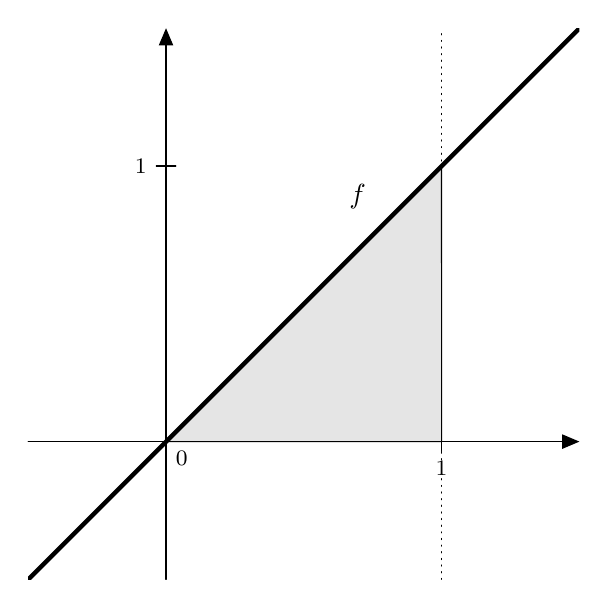
\begin{tikzpicture}[scale=3.5,line cap=round,line join=round,>=triangle 45,x=1.0cm,y=1.0cm]
\draw[->,color=black] (-0.5,0) -- (1.5,0);
\foreach \x in {,1}
\draw[shift={(\x,0)},color=black] (0pt,1pt) -- (0pt,-1pt) node[below] {\footnotesize $\x$};
\draw[->,color=black] (0,-0.5) -- (0,1.5);
\foreach \y in {,1}
\draw[shift={(0,\y)},color=black] (1pt,0pt) -- (-1pt,0pt) node[left] {\footnotesize $\y$};
\draw[color=black] (0,0) node[anchor=north west] {\footnotesize $0$};
\clip(-0.5,-0.5) rectangle (1.5,1.5);
\draw[color=black,fill=black,fill opacity=0.1, smooth,samples=50,domain=0.0:1.0]
plot(\x,{\x}) -- (1,0) -- (0,0) -- cycle;
\draw[line width=1.6pt, smooth,samples=100,domain=-0.5:1.5] plot(\x,{(\x)});
\draw [dotted] (1,-0.5) -- (1,1.5);
\draw (0.63,0.97) node[anchor=north west] {$f$};
\end{tikzpicture}
\end{center}

\begin{itemize}
  \item We delen $[0,1]$ op in $n$ deelintervallen van lengte $\Delta x=\dfrac{1}{n}$:
  $$[0,\dfrac{1}{n}],\, [\dfrac{1}{n},\dfrac{2}{n}],\, [\dfrac{2}{n},\dfrac{3}{n}],\, \ldots,\, [\dfrac{n-2}{n},\dfrac{n-1}{n}],\, [\dfrac{n-1}{n},1]$$
  \item Op een deelinterval $[\dfrac{k-1}{n},\dfrac{k}{n}]$:
  \begin{itemize}
    \item kleinste waarde: $\min_k f = \dfrac{k-1}{n}$
    \item grootste waarde: $\max_k f = \dfrac{k}{n}$
  \end{itemize}
  \item Onder- en bovensom:
  \begin{itemize}
    \item ondersom: $s_n=\sum^n_{k=1}\min_k f \cdot \Delta x=\sum^n_{k=1}\dfrac{k-1}{n}\cdot\dfrac{1}{n}=\dfrac{n-1}{2n}$
    \item bovensom: $S_n=\sum^n_{k=1}\max_k f \cdot \Delta x=\sum^n_{k=1}\dfrac{k}{n}\cdot\dfrac{1}{n}=\dfrac{n+1}{2n}$
  \end{itemize}
  \item Limieten berekenen:
  $$\lim_{n\to+\infty}s_n=\lim_{n\to+\infty}\dfrac{n-1}{2n}=\dfrac{1}{2}$$
  $$\lim_{n\to+\infty}S_n=\lim_{n\to+\infty}\dfrac{n+1}{2n}=\dfrac{1}{2}$$
  \item Besluit:
  $$\int_0^1 x\;dx=\dfrac{1}{2}$$
\end{itemize}

\subsection{Eigenschappen}

\begin{itemize}
  \item Gelijke grenzen: $a=b \Rightarrow \mbox{opp}=0$
  $$\int_a^a f(x)\;dx = 0$$
  \item Wisselen van de grenzen: $a\leftrightarrow b \Rightarrow \Delta x \mbox{ verandert van teken}$
  $$\int_a^b f(x)\;dx = -\int_b^a f(x)\;dx$$
  \item Opsplitsen van de integraal: $\forall c\in[a,b]:$
  $$\int_a^b f(x)\;dx = \int_a^c f(x)\;dx + \int_c^b f(x)\;dx$$
  \item Lineariteit van de integraal: $\alpha, \beta\in\mathbb{R}$
  $$\int_a^b \alpha f(x) + \beta g(x)\;dx = \alpha \int_a^b f(x) \;dx+ \beta \int_a^b g(x)\;dx$$
\end{itemize}

\subsection{Primitieve functie}

We voeren een nieuwe notatie in
$$[F(x)]_a^b = F(b) - F(a)$$
en lezen dit als we berekenen $F$ van $a$ naar $b$.

\begin{oefening}
Bereken
\begin{multicols}{2}
\begin{enumerate}[(a)]
  \itemsep.5em
  \item $\displaystyle\left[2x-3\right]_1^3$
  \item $\displaystyle\left[x^2\right]_0^4$
  \item $\displaystyle\left[\ln x\right]_1^e$
  \item $\displaystyle\left[\ln x\right]_0^e$
\end{enumerate}
\end{multicols}
\end{oefening}

\begin{oefening}
\begin{enumerate}[(a)]
  \item Beschouw de functies
  $$f(x)=2 \mbox{ en } F(x)=2x$$
  \begin{itemize}
    \item Bereken de oppervlakte begrepen tussen $y=f(x),\;y=0,\;x=1,\;x=4$
    \item Bereken $[F(x)]_1^4$
    \item Wat is het verband tussen $f$ en $F$
  \end{itemize}
  \item Beschouw de functies
  $$f(x)=x \mbox{ en } F(x)=\dfrac{x^2}{2}$$
  \begin{itemize}
    \item Bereken de oppervlakte begrepen tussen $y=f(x),\;y=0,\;x=0,\;x=4$
    \item Bereken $[F(x)]_0^4$
    \item Wat is het verband tussen $f$ en $F$
  \end{itemize}
  \item Beschouw de functies
  $$f(x)=x \mbox{ en } F(x)=\dfrac{x^2}{2}$$
  \begin{itemize}
    \item Bereken de oppervlakte begrepen tussen $y=f(x),\;y=0,\;x=2,\;x=5$
    \item Bereken $[F(x)]_2^5$
    \item Wat is het verband tussen $f$ en $F$
  \end{itemize}
\end{enumerate}
\end{oefening}

We krijgen volgende definitie:

T.o.v. een orthonormaal assenstelsel is de oppervlakte $S$ begrepen tussen $y=f(x),\;y=0,\;x=a,\;x=b$ gelijk aan
$$S=\left[F(x)\right]_a^b \mbox{ met } F'(x)=f(x)\;.$$ We noemen $F$ {\em een} {\bf primitieve functie} van $f$.

\begin{oefening}
Bepaal {\em alle} primitieve functies van
\begin{exlist}{2}
  \item $f(x)=5$
  \item $f(x)=7$
  \item $f(x)=0$
  \item $f(x)=2x$
  \item $f(x)=x$
  \item $f(x)=3x^2$
  \item $f(x)=x^2$
  \item $f(x)=x^n$ met $n\in\mathbb{R}\setminus\{-1\}$
\end{exlist}
\end{oefening}

Merk op dat elke functie $f$ oneindig veel primitieve functies $F$ heeft.

\subsection{Een bepaalde integraal berekenen}

\paragraph{Stelling}

Is $f$ continu in $[a,b]$ en is $F$ een primitieve functie van $f$ in $[a,b]$ dan geldt
$$\int_a^b f(x)\;dx = [F(x)]_a^b$$

\paragraph*{Gevolg}
$$\int_a^b x^n\;dx = \left[\dfrac{x^{n+1}}{n+1}\right]_a^b \mbox{ met } n\in\mathbb{R}\setminus\{-1\}$$

\begin{oefening}
Bereken
\begin{multicols}{3}
\begin{enumerate}[(a)]
  \itemsep1em
  \item $\displaystyle \int_0^2 x^3 \;dx$
  \item $\displaystyle \int_{-1}^{1} x^2 \;dx$
  \item $\displaystyle \int_1^3 x^4 \;dx$
  \item $\displaystyle \int_{-4}^4 \;dx$
  \item $\displaystyle \int_{-1}^{1} x \;dx$
  \item $\displaystyle \int_{-1}^{1} |x| \;dx$
\end{enumerate}
\end{multicols}
\end{oefening}

\paragraph*{Integraal van een veeltermfunctie}
M.b.v. de lineariteit van een bepaalde integraal kunnen we de bepaalde integraal van een veeltermfunctie berekenen, bijvoorbeeld
\begin{align*}
  \int_1^3 2x^3-3x+1 \;dx &= \int_1^3 2x^3 \;dx + \int_1^3 -3x \;dx + \int_1^3 1 \;dx\\
                       &= 2\int_1^3 x^3 \;dx - 3\int_1^3 x \;dx + \int_1^3 \;dx\\
                       &= 2\cdot\left[\dfrac{x^4}{4}\right]_1^3
                         - 3\cdot\left[\dfrac{x^2}{2}\right]_1^3
                         + \left[x\right]_1^3\\
                       &= 2\cdot \left(\dfrac{81}{4}-\dfrac{1}{4}\right)
                         - 3\cdot \left(\dfrac{9}{2}-\dfrac{1}{2}\right)
                         + \left(3-1\right)\\
                       &= 40 - 12 + 2\\
                       &= 30
\end{align*}
of veel korter!
\begin{align*}
  \int_1^3 2x^3-3x+1 \;dx &= \cdot\left[2\cdot\dfrac{x^4}{4} - 3\cdot\dfrac{x^2}{2} + x\right]_1^3\\
                       &= (2\cdot \dfrac{81}{4} - 3\cdot \dfrac{9}{2} + 3)
                         - (2\cdot \dfrac{1}{4} - 3\cdot \dfrac{1}{2} + 1)\\
                       &= 30
\end{align*}

\begin{oefening}
Bereken volgende bepaalde integralen
\begin{multicols}{2}
\begin{enumerate}[(a)]
\itemsep1em
  \item $\displaystyle \int_{-1}^2 (3x^2+2x-1)\;dx$
  \item $\displaystyle \int_{-4}^3 (6x^8+12x^5-\dfrac{1}{2}x^2)\;dx$
  \item $\displaystyle \int_{0}^5 (3x+5)^2\;dx$
  \item $\displaystyle \int_1^2 \dfrac{1}{x^2}\;dx$
  \item $\displaystyle \int_{-3}^{-1} \dfrac{4}{3x^3} \;dx$
  \item $\displaystyle \int_4^{16} \sqrt{x} \;dx$
  \item $\displaystyle \int_8^{27} \sqrt[3]{x} \;dx$
  \item $\displaystyle \int_2^8 \sqrt{2x} \;dx$
  \item $\displaystyle \int_8^{27} \dfrac{1}{\sqrt[3]{x}} \;dx$
  \item $\displaystyle \int_3^{16/3} \dfrac{x}{\sqrt{3x}} \;dx$
  \item $\displaystyle \int_{0}^3 (x+1)^3\;dx$
  \item $\displaystyle \int_{0}^2 (x+2)^6\;dx$
  \item $\displaystyle \int_{-1}^3 \dfrac{x^2+x}{x}\;dx$
  \item $\displaystyle \int_{-4}^4 \dfrac{x^3+2x^2+2}{4x^2}\;dx$
  \item $\displaystyle \int_{4}^0 \sqrt{x}(x-2)\;dx$
\end{enumerate}
\end{multicols}
\end{oefening}

\begin{oefening}
Bereken
\begin{multicols}{2}
\begin{enumerate}[(a)]
\itemsep1em
  \item $\displaystyle \int_1^2 y^2+y^{-2} \;dy$
  \item $\displaystyle \int_{-1}^2 y^2+y^{-2} \;dy$
  \item $\displaystyle \int_1^2 \dfrac{2\omega^5-\omega^2+3}{\omega^2} \;d\omega$
  \item $\displaystyle \int_{25}^{-10} \;dR$
\end{enumerate}
\end{multicols}
\end{oefening}

\begin{oefening} % source http://tutorial.math.lamar.edu/Classes/CalcI/ComputingDefiniteIntegrals.aspx
Gegeven
$$f(x)=\begin{cases}6 & \mbox{ if } x > 1\\3x^2 & \mbox{ if } x \leq 1\\\end{cases}$$
Bepaal
$$\displaystyle \int_{10}^{22} f(x) \;dx \qquad\mbox{ en }\qquad \displaystyle \int_{-2}^{3} f(x) \;dx$$
\end{oefening}

\cleardoublepage
\section{Oppervlakteberekeningen}

\subsection{Verband bepaalde integraal en oppervlakte}

We houden rekening met 4 gevallen om de oppervlakte van een functie $f$ in een interval $[a,b]$ te berekenen m.b.v. een integraal:
\begin{itemize}
  \item $a<b$ en $f(x)\geq0$ in $[a,b]$
  \begin{align*}
    \int_a^b f(x)\; dx \geq 0 & \Rightarrow S=\int_a^b f(x)\; dx
  \end{align*}
  \item $a<b$ en $f(x)\leq0$ in $[a,b]$
  \begin{align*}
    \int_a^b f(x)\; dx \leq 0 & \Rightarrow S=-\int_a^b f(x)\; dx  \\
                        & \Rightarrow S=|\int_a^b f(x)\; dx| \\
  \end{align*}
  \item $a>b$ en $f(x)\geq0$ in $[a,b]$
  \begin{align*}
    \int_a^b f(x)\; dx \leq 0 & \Rightarrow S=-\int_a^b f(x)\; dx  \\
                        & \Rightarrow S=|\int_a^b f(x)\; dx| \\
  \end{align*}
  \item $a>b$ en $f(x)\leq0$ in $[a,b]$
  \begin{align*}
    \int_a^b f(x)\; dx \geq 0 & \Rightarrow S=\int_a^b f(x)\; dx
  \end{align*}
\end{itemize}

\subsubsection*{Besluit}

Ten opzichte van een orthonormaal assenstelsel geldt dat we het oppervlakte van het deel va het vlak begrensd door $y=f(x)$, $y=0$, $x=a$, $x=b$ kunnen berekenen met
$$S = |\int_a^b f(x)\;dx|$$
als $f$ geen nulwaarden heeft tussen $a$ en $b$.

\subsubsection*{Opmerking}

Heeft $f$ wel nulwaarden tussen $a$ en $b$ dan kunnen we theoretisch gezien de berekening maken met behulp van
$$S = \int_a^b |f(x)|\;dx$$
wat we in de praktijk zullen doen door $f$ te spliten bij de nulwaarden, en de berekening apart zullen doen.

\begin{oefening}
Bepaal de oppervlakte tussen
\begin{enumerate}[(a)]
\itemsep1em
  \item $\displaystyle y=x^2,\quad y=0,\quad x=0, \quad x=2$
  \item $\displaystyle y=x^2-6x,\quad y=0,\quad x=2, \quad x=4$
  \item $\displaystyle y=\sqrt{x},\quad y=0,\quad x=0, \quad x=9$
  \item $\displaystyle y=\sqrt[3]{x},\quad y=0,\quad x=-4, \quad x=4$
  \item $\displaystyle y=\dfrac{x^2-1}{x^2},\quad y=0,\quad x=-3, \quad x=-1$
  \item $\displaystyle y=\dfrac{x^2-4}{x^2},\quad y=0,\quad x=1, \quad x=6$
  \item $\displaystyle y=x(x-3),\quad y=0,\quad x=0, \quad x=5$
\end{enumerate}
\end{oefening}

\begin{oefening}
Bepaal de oppervlakte tussen de gegeven kromme en de $x$-as
%\begin{multicols}{2}
\begin{enumerate}[(a)]
\itemsep1em
  \item $\displaystyle y=4x-x^2$
  \item $\displaystyle y=4x-x^3$
  \item $\displaystyle y=-x^3+5x^2-7x+3$
  \item $\displaystyle y=4x^4-8x^3-12x^2+16x+16$
\end{enumerate}
%\end{multicols}
\end{oefening}

\subsection{Berekenen van de oppervlakte tussen twee krommen}

Veronderstel dat we de oppervlakte $S$ berekenen tussen de krommen die voorgesteld worden met de functies
$$y=f(x) \text{ en } y=g(x)$$
\begin{itemize}
\item We maken een schets van de twee functies $f$ en $g$ in éénzelfde assenstelsel.
\item We zoeken de snijpunten van de twee krommen, we lossen dus
  $$f(x)-g(x)=0$$
  op naar $x$. Dit worden de integratiegrenzen $a$ en $b$.
\item De gezochte oppervlakte is dan
  $$S = \int_a^b (f(x)-g(x))\; dx$$
  op voorwaarde dat $f(x) \geq g(x)$ is in $[a,b]$.
\end{itemize}


\begin{oefening}
Bepaal de oppervlakte tussen $f$ en $g$
\begin{enumerate}[(a)]
\itemsep1em
  \item $f(x)=x^2$ en $g(x)=2x$
  \item $f(x)=x$ en $g(x)=2x-x^2$
\end{enumerate}
\end{oefening}

\begin{oefening}
Bepaal de oppervlakte tussen
\begin{enumerate}[(a)]
\itemsep1em
  \item $x=y^3-26y+10$ en $x=40-6y^2-y^3$
  \item $x=|y|$ en $x=1-|y|$
  \item $y=|x|$ en $y=x^2-6$
  \item $y=\sqrt{x}$ en $y=x^2$
\end{enumerate}
\end{oefening}

\subsection{Berekenen van de oppervlakte van een gebied}

Elke situatie kan anders zijn. Begin met het tekenen van een schets en leidt hier de grenzen en integrand uit af.

\begin{oefening}
Bepaal de oppervlakte tussen
\begin{enumerate}[(a)]
\itemsep1em
  \item $\displaystyle y=\sqrt{x},\quad y=\sqrt{x+1},\quad x=0, \quad x=4$
\end{enumerate}
\end{oefening}

\cleardoublepage
\section{Berekenen van integralen}

\subsection{Onbepaalde integraal}

\subsubsection*{Definities}

We kunnen het integreren, naast het berekenen van een oppervlakte, ook zien als een bewerking (operator) die we toepassen op een functie $f$ om een andere fuctie $F$ te vinden, namelijk een primitieve van die functie.

We herhalen de definitie van primitieve:
\begin{mdframed}
  De functie $F$ is een {\bf primitieve functie} van $f$ als
  $$F' = f$$
\end{mdframed}

En definiëren nu de operator die op zoek gaat naar die primitieve:
\begin{mdframed}
  De {\bf onbepaalde integraal} van een functie $f$ is de verzameling van alle primitieve functies $F$ van $f$:
  $$\int f(x)\;dx = F(x) + c$$
  met $c \in \mathbb{R}$.
\end{mdframed}

\subsubsection*{Voorbeelden}

\begin{enumerate}[(a)]
\item $\displaystyle \int x^4\;dx = \dfrac{x^5}{5} + c$ want $\displaystyle \left(\dfrac{x^5}{5} + c \right)' = x^4$
\item $\displaystyle \int \cos x\;dx = \sin x + c$ want $\displaystyle \left(\sin x + c \right)' = \cos x$
\item $\displaystyle \int \dfrac{1}{x} \;dx = \ln|x| + c$ want $\displaystyle \left(\ln|x| + c \right)' = \dfrac{1}{x}$
\end{enumerate}

\subsubsection*{Eigenschappen}

\begin{itemize}
\item Integreren en differentiëren zijn inverse operaties:\\
  Stelling: $\displaystyle \left(\int f(x) \;dx \right)'=f(x)$\\
  Bewijs:
  \begin{align*}
    LL &= \left(\int f(x) \;dx \right)'\\
       &= \left(F(x) + c \right)'\\
       &= F'(x)\\
       &= f(x)\\
       &= RL
  \end{align*}
  Stelling: $\displaystyle \int dF(x) \;dx = F(x) + c$\\
  Bewijs:
  \begin{align*}
    LL &= \int dF(x) \;dx\\
       &= \int F'(x) \;dx\\
       &= \int f(x) \;dx\\
       &= F(x) + c\\
       &= RL
  \end{align*}
\item Lineariteit van de onbepaalde integraal:
  $$\int \alpha \cdot f(x) + \beta \cdot g(x)\;dx = \alpha \int f(x)\;dx + \beta \int g(x)\;dx$$
\end{itemize}

\subsection{Basisformules van de integraalrekening}

De basisintegralen volgen uit de lijst van de basisafgeleiden, de afgeleide van de functie in het rechterlid is namelijk gelijk aan de integrand. We hebben telkens een {\bf integratieconstante} $C\in\mathbb{R}$.

\subsubsection*{Basisintegralen}
\begin{mdframed}
\begin{multicols}{2}
\begin{align*}
  \int \;dx &= x + C\\
  \int x^n \;dx &= \dfrac{x^{n+1}}{n+1} + C\\
  \int \dfrac{1}{x} \;dx &= \ln|x| + C
\end{align*}
\begin{align*}
  \int e^x \;dx &= e^x + C\\
  \int a^x \;dx &= \dfrac{a^x}{\ln a} + C\\
  \int \sin x \;dx &= -\cos x + C\\
  \int \cos x \;dx &= \sin x + C
\end{align*}
\end{multicols}
\end{mdframed}

\needspace{3cm}
\subsubsection*{Voorbeelden}

\begin{enumerate}[(a)]
\item $\displaystyle \int x^6 \;dx = \dfrac{x^7}{7} + C$
\item $\displaystyle \int \dfrac{1}{x^3} \;dx = -\dfrac{1}{2x^2} + C$
\item $\displaystyle \int \sqrt{x^3} \;dx = \dfrac{2}{5}\sqrt{x^5} + C$
\item $\displaystyle \int 2^x \;dx = \dfrac{2^x}{\ln 2} + C$
\item $\displaystyle \int (2x^2 - 4x + 1) \;dx = x^3 - 2x^2 + x + C$
\item $\displaystyle \int (3 \sin x - 2 \cos x) \;dx = -3 \cos x - 2 \sin x + C$
\end{enumerate}

\begin{oefening}
  Werk uit
  \begin{multicols}{2}
    \begin{enumerate}[(a)]
      \itemsep.5em
    \item $\displaystyle \int \;dx$
    \item $\displaystyle \int x^2 \;dx$
    \item $\displaystyle \int x^\pi \;dx$
    \item $\displaystyle \int (4x^3 + 2x) \;dx$
    \item $\displaystyle \int (x^3 + x^2 + x + 1) \;dx$
    \end{enumerate}
  \end{multicols}
\end{oefening}

\begin{oefening}
  Werk uit
  \begin{multicols}{2}
    \begin{enumerate}[(a)]
      \itemsep.5em
    \item $\displaystyle \int \dfrac{1}{x^3} \;dx$
    \item $\displaystyle \int \left(\dfrac{8}{x^4} - \dfrac{3}{x^2}\right) \;dx$
    \item $\displaystyle \int \sqrt[3]{x} \;dx$
    \item $\displaystyle \int \dfrac{1}{\sqrt[3]{x}} \;dx$
    \item $\displaystyle \int \dfrac{\sqrt[3]{x}}{x} \;dx$
    \item $\displaystyle \int \dfrac{\sqrt[4]{x}}{\sqrt[3]{x}} + \dfrac{x^3}{x^2} \;dx$
    \end{enumerate}
  \end{multicols}
\end{oefening}

\begin{oefening}
  Werk uit
  \begin{multicols}{2}
    \begin{enumerate}[(a)]
      \itemsep.5em
    \item $\displaystyle \int \dfrac{2}{x} \;dx$
    \item $\displaystyle \int \dfrac{-x^2 + x - 1}{x} \;dx$
    \item $\displaystyle \int 5^x \;dx$
    \item $\displaystyle \int 2^x \cdot 3^x \;dx$
    \item $\displaystyle \int \dfrac{e^x}{e} \;dx$
    \end{enumerate}
  \end{multicols}
\end{oefening}

\begin{oefening} {\scriptsize \em IJkingsproef industrieel ingenieur}\\
Bereken
$$\int \dfrac{(1+x)^2}{\sqrt{x}}\;dx$$
\begin{enumerate}[(A)]
\itemsep.5em
  \item $x^{5/2}+x^{3/2}+x^{1/2} + C$
  \item $\dfrac{(x+1)^3}{3\sqrt{x}} + C$
  \item $\dfrac{2}{5}x^{5/2}+\dfrac{2}{3}x^{3/2}+2x^{1/2} + C$
  \item $\dfrac{2}{5}x^{5/2}+\dfrac{4}{3}x^{3/2}+2x^{1/2} + C$
\end{enumerate}
\end{oefening}

\subsection{Substitutiemethode}

\subsubsection{$t=x+a$ met $a\in\mathbb{R}$}

\begin{align*}
  t = x+a \Rightarrow dt &= d(x+a)\\ &= (x+a)'\cdot dx \\ &= dx
\end{align*}

\vspace{-1cm}
\subsubsection*{Voorbeeld 1}
\begin{align*}
  \int \left(x+4\right)^8\cdot dx
  &= \int t^8 \cdot dt \qquad\qquad\mbox{subs }t=x+3 \Rightarrow dx = dt\\
  &= \dfrac{t^9}{9} + C\\
  &= \dfrac{(x+3)^9}{9} + C
\end{align*}
Of korter genoteerd:
\begin{align*}
  \int \left(x+4\right)^8\cdot dx &= \int (x+4)^8 \cdot d(x+4)\\
  &= \dfrac{(x+3)^9}{9} + C
\end{align*}

\vspace{-1cm}
\subsubsection*{Voorbeeld 2}
\begin{align*}
  \int \dfrac{1}{x-5} \cdot dx &= \int \dfrac{1}{t} \cdot dt \qquad\qquad\mbox{subs }t=x-5 \Rightarrow dx = dt\\
  &= \ln|t| + C\\
  &= \ln|x-5| + C
\end{align*}
Of korter:
\begin{align*}
  \int \dfrac{1}{x-5} \cdot dx &= \int \dfrac{1}{x-5} \cdot d(x-5)\\
  &= \ln|x-5| + C
\end{align*}

\begin{oefening}
  Bereken
  \begin{multicols}{2}
  \begin{enumerate}[(a)]
  \item $\displaystyle\int \sqrt{x+6} \;dx$
  \item $\displaystyle\int e^{x+9} \;dx$
  \item $\displaystyle\int \dfrac{1}{\cos^2(x-1)} \;dx$
  \item $\displaystyle\int \dfrac{1}{3(x-8)^4} \;dx$
  \item $\displaystyle\int (2x-2)\cdot\sqrt{x-1} \;dx$
  \end{enumerate}
\end{multicols}
\end{oefening}

\subsubsection{$t=ax+b$ met $a\in\mathbb{R}_0, b\in\mathbb{R}$}

\begin{alignat*}{2}
  t = ax+b &&\Rightarrow dt &= d(ax+b)\\ && &= (ax+b)'\cdot dx \\ && &= a \cdot dx\\
           &&\Leftrightarrow dx &= \dfrac{1}{a} \cdot dt
\end{alignat*}

\subsubsection*{Voorbeeld 1}
\begin{align*}
  \int \cos(2x) \;dx
  &= \int \cos t \cdot \dfrac{1}{2} \;dt \qquad\qquad\mbox{subs }t=2x \Rightarrow dt = 2dx \Rightarrow dx = \dfrac{1}{2} \;dt\\
  &= \dfrac{1}{2} \int \cos t \;dt\\
  &= \dfrac{1}{2} \sin t + C\\
  &= \dfrac{1}{2} \sin 2x + C
\end{align*}
Of korter genoteerd:
\begin{align*}
  \int \cos(2x) \;dx &= \int \cos 2x \cdot \dfrac{1}{2} \;d(2x)\\
  &= \dfrac{1}{2} \sin 2x + C
\end{align*}

\subsubsection*{Voorbeeld 2}
\begin{align*}
  \int \sqrt{4x-7} \;dx
  &= \int \sqrt{t} \cdot \dfrac{1}{4} \;dt \qquad\qquad\mbox{subs }t=4x-7 \Rightarrow dt = 4dx \Rightarrow dx = \dfrac{1}{4} \;dt\\
  &= \dfrac{1}{4} \int t^{1/2} \;dt\\
  &= \dfrac{1}{4} \cdot \dfrac{t^{3/2}}{3/2} + C\\
  &= \dfrac{1}{6} \cdot t\cdot t^{1/2} + C\\
  &= \dfrac{1}{6} \cdot t\cdot \sqrt{t} + C\\
  &= \dfrac{1}{6} (4x-7)\cdot \sqrt{4x-7} + C\\
\end{align*}

\begin{oefening}
  Bereken
  \begin{multicols}{2}
  \begin{enumerate}[(a)]
  \item $\displaystyle\int \dfrac{1}{3x-8} \;dx$
  \item $\displaystyle\int e^{5x+3} \;dx$
  \item $\displaystyle\int \dfrac{1}{\sqrt[3]{(5x+7)^2}} \;dx$
  \item $\displaystyle\int 5\sin(3-x) \;dx$
  \item $\displaystyle\int 2^{8x-3} \;dx$
  \item $\displaystyle\int \dfrac{(2x+1)^2 \cdot \sqrt{2x+1}}{\sqrt[3]{(2x+1)^2}} \;dx$
  \item $\displaystyle\int \dfrac{\sqrt[3]{4-5x}}{(5x-4)^4} \;dx$
  \item $\displaystyle\int \dfrac{3x+2}{3x+1} \;dx$
  \end{enumerate}
\end{multicols}
\end{oefening}

\subsubsection{Integrand $f'(x)/f(x)$}

De integrand bestaat dus uit een teller die de afgeleide is van de noemer.

\begin{alignat*}{2}
  \mbox{subst } t = f(x) &&\Rightarrow dt &= df(x)\\
  &&               &= \dfrac{df(x)}{dx} \cdot dx \\
  &&               &= f'(x) \cdot dx\\
  &&\Rightarrow \int \dfrac{f'(x)}{f(x)} \;dx &= \int \dfrac{1}{t} \;dt\\
  &&                                          &= \ln |t| + C\\
  &&                                          &= \ln |f(x)| + C
\end{alignat*}

\vspace{-1cm}
\subsubsection*{Voorbeeld 1}
\begin{align*}
  \int \dfrac{2x}{x^2+1} \;dx
  &= \int \dfrac{dt}{t} && \mbox{subs }t=x^2+1 \Rightarrow dt = 2x\;dx\\
  &= \ln |t| +C\\
  &= \ln |x^2+1| + C\\
  &= \ln(x^2+1) + C  &&\mbox{ want } x^2+1 > 0 \;  \forall x \in \mathbb{R}
\end{align*}

\vspace{-1cm}
\subsubsection*{Voorbeeld 2}
\begin{align*}
  \int \tan \;dx &= \int \dfrac{\sin x}{\cos x} \;dx\\
  &= - \int \dfrac{dt}{t} &&\mbox{subs }t=\cos x \Rightarrow dt = -\sin x\;dx\\
  &= - \ln |t| +C\\
  &= - \ln |\cos x| + C\\
\end{align*}

\vspace{-1cm}
\begin{oefening}
  Bereken
  \begin{multicols}{2}
  \begin{enumerate}[(a)]
  \item $\displaystyle\int \dfrac{x^2}{x^3+1} \;dx$
  \item $\displaystyle\int \dfrac{2x+1}{x^2+x+3} \;dx$
  \item $\displaystyle\int \dfrac{12x}{x^2-5} \;dx$
  \item $\displaystyle\int \dfrac{x^2}{13-x^3} \;dx$
  \item $\displaystyle\int \dfrac{1-\sin x}{x+\cos x} \;dx$
  \item $\displaystyle\int \dfrac{e^x}{e^x-9} \;dx$
  \item $\displaystyle\int \dfrac{1}{(2x+5) \cdot \ln(2x+5)} \;dx$
  \end{enumerate}
\end{multicols}
\end{oefening}

\subsubsection{Andere substituties}

Geen algemene regel, wat je kiest voor de substitutie $t$ hangt af van de integrand.

\subsubsection*{Voorbeeld 1}
\begin{align*}
  \int \sin^5x \cdot \cos x \cdot \;dx
  &= \int t^5 \;dt \qquad\qquad\mbox{subs }t=\sin x \Rightarrow dt = \cos x \;dx\\
  &= \dfrac{t^6}{6} +C\\
  &= \dfrac{1}{6}\sin^6 x + C
\end{align*}

\subsubsection*{Voorbeeld 2}
\begin{align*}
  \int x \cdot \sqrt{x+3} \;dx
  &= \int (t-3) \cdot \sqrt{t} \cdot \;dt \qquad\qquad\mbox{subs }t=x+3 \Rightarrow dt = dx\\
  &= \int t\cdot t^{1/2} - 3\cdot t^{1/2} \;dt\\
  &= \int t^{3/2} \;dt - 3 \int t^{1/2} \;dt\\
  &= \dfrac{t^{5/2}}{5/2} - 3\cdot \dfrac{t^{3/2}}{3/2} + C\\
  &= \frac{2}{5}t^2\sqrt{t} - 2 t \sqrt{t} + C\\
  &= 2t\sqrt{t}(\frac{t}{5}-1) + C\\
  &= 2(x+3)\sqrt{x+3}\left(\frac{x+3}{5}-1\right) + C\\
  &= \dfrac{2}{5}(x+3)\sqrt{x+3}\left(x-2\right) + C\\
\end{align*}

\subsubsection*{Voorbeeld 3}

Voor het volgende voorbeeld herinneren we ons nog de $t$-formules waarbij $t=\tan\dfrac{x}{2}$
$$\sin x = \dfrac{2t}{1+t^2} \qquad \cos x = \dfrac{1-t^2}{1+t^2} \qquad \tan x = \dfrac{2t}{1-t^2}$$
en dat we m.b.v. de grondformule (beide leden delen door $\cos^2\theta$)
$$\cos^2\theta + \sin^2\theta = 1 \Leftrightarrow 1 + \tan^2\theta = \dfrac{1}{\cos^2\theta}$$
bekomen.

Bereken $\displaystyle\int \dfrac{dx}{\sin x}$
\begin{alignat*}{2}
  \mbox{stel } t =\tan \dfrac{x}{2}\\
  \Rightarrow &&\;\sin x &= \dfrac{2t}{1+t^2} \qquad \mbox{herinner je de $t$-formule}\\
  \Rightarrow &&dt &= d\left(\tan\dfrac{x}{2}\right)\\
  && &=\dfrac{1}{\cos^2\dfrac{x}{2}} \; d\left(\dfrac{x}{2}\right)\\
  && &=\dfrac{1}{2 \cdot \cos^2\dfrac{x}{2}} \; dx\\
  \Leftrightarrow &&dx &= 2 \cdot \cos^2\dfrac{x}{2} \; dt\\
  && &= \dfrac{2}{1+\tan^2\dfrac{x}{2}} \; dt \qquad \mbox{herinner je de grondformule}\\
  && &= \dfrac{2}{1+t^2} \; dt \qquad \mbox{herinner je wat $t$ is in de $t$-formules}\\
\end{alignat*}
En dus
\begin{align*}
  \int \dfrac{dx}{\sin x}
  &= \int \dfrac{1}{\text{\footnotesize$\dfrac{2t}{1+t^2}$}} \cdot \dfrac{2}{1+t^2} \;dt\\
  &= \int \dfrac{1}{t}\;dt\\
  &= \ln|t| + C\\
  &= \ln|\tan\dfrac{x}{2}| + C\\
\end{align*}

\subsubsection{Gemengde oefeningen}

\begin{oefening}
  Bereken
  \begin{multicols}{2}
  \begin{enumerate}[(a)]
  \item $\displaystyle\int (x-2)^5 \;dx$
  \item $\displaystyle\int \dfrac{1}{2x} \;dx$
  \item $\displaystyle\int \dfrac{2x-1}{x^2-x}  \;dx$
  \item $\displaystyle\int \dfrac{3x-1}{\sqrt{3x-1}}  \;dx$
  \item $\displaystyle\int \dfrac{1}{x \ln 2x}  \;dx$
  \item $\displaystyle\int e^{2x+3} \;dx$
  \item $\displaystyle\int \dfrac{6x^2+x}{4x^3-x^2+3} \;dx$
  \item $\displaystyle\int \cos (-5x) \;dx$
  \item $\displaystyle\int \dfrac{1}{\sin^2(-x)} \;dx$
  \item $\displaystyle\int \dfrac{2}{\cos^2(2x)\tan(2x)} \;dx$
  \end{enumerate}
\end{multicols}
\end{oefening}

\begin{oefening}
  Bereken
  \begin{multicols}{2}
  \begin{enumerate}[(a)]
  \item $\displaystyle\int (4x-2)^3 \;dx$
  \item $\displaystyle\int \dfrac{1}{\cos^2(3x)} \;dx$
  \item $\displaystyle\int \dfrac{6x^2-10}{x^3-5x+2} \;dx$
  \item $\displaystyle\int \sin(-2x) \;dx$
  \item $\displaystyle\int \dfrac{3}{\sin^2(3x) \cdot \cot(3x)}  \;dx$
  \end{enumerate}
\end{multicols}
\end{oefening}

%\pagebreak
\subsection{Partiële integratie}

\subsubsection{Stelling}


\begin{mdframed}
Als de functies $f$ en $g$ differentieerbaar zijn in alle beschouwde punten, dan geldt
$$\int f(x) \cdot \dg(x) = f(x) \cdot g(x) - \int g(x) \cdot df(x)$$
\end{mdframed}

\subsubsection{Voorbeelden}

\subsubsection*{Voorbeeld 1}
Bereken
$$\int \cos(x)\cdot x\;dx$$

We berekenen eerst
\begin{alignat*}{3}
  f(x) &= \cos x \qquad & dg(x) &= x\cdot dx\\
  df(x) &= - \sin x \; dx \qquad & g(x) &= \dfrac{1}{2} x^2
\end{alignat*}

Dus
\begin{align*}
  \int \cos(x)\cdot x\;dx
  &\overset{\text{PI}}{=} \cos x \cdot \dfrac{1}{2}x - \int \dfrac{1}{2} x^2 \cdot (-\sin x) \cdot dx\\
  &= \dfrac{1}{2}x \cos x + \dfrac{1}{2} \underbrace{\int x^2 \cdot \sin x \; dx}_{\text{moeilijker}}
\end{align*}

Maar nu is de integraal die overblijft in het rechterlid moeilijker dan de oorspronkelijke integraal. We zijn geen opgevers en proberen opnieuw, maar nu met een andere keuze voor $f$ en $dg$ want we kunnen de integraal ook schrijven als
$$\int \cos(x)\cdot x\;dx = \int x\cdot \cos x\;dx$$

We berekenen nu dus
\begin{alignat*}{3}
  f(x) &= x \qquad & dg(x) &= \cos x\cdot dx\\
  df(x) &= dx \qquad & g(x) &= \sin x
\end{alignat*}

\vspace{-0.5cm}
En dus
\begin{align*}
  \int x \cdot \cos x \;dx
  &\overset{\text{PI}}{=} x\cdot \sin x - \int \sin x \cdot dx\\
  &= x\cdot \sin x + \cos x + C\\
\end{align*}

\subsubsection*{Voorbeeld 2}
Bereken $\displaystyle I=\int x\cdot \sin(3x) \cdot dx$
\begin{alignat*}{3}
  f(x) &= x \qquad & dg(x) &= \sin 3x\cdot dx\\
  df(x) &= dx \qquad & g(x) &= -\dfrac{1}{3} \cos 3x
\end{alignat*}
\begin{align*}
  I
  &\overset{\text{PI}}{=} x\cdot (-\dfrac{1}{3}\cos 3x) - \int (-\dfrac{1}{3})\cos 3x \cdot dx\\
  &= -\dfrac{1}{3}x\cos 3x + \dfrac{1}{3} \int \cos 3x \; dx\\
  &= -\dfrac{1}{3}x\cos 3x + \dfrac{1}{3} \int \cos t \; \dfrac{1}{3}dt \qquad t=3x\Rightarrow dt=3dx \Rightarrow dx=\dfrac{1}{3}dt\\
  &= -\dfrac{1}{3} x \cos 3x + \dfrac{1}{9} \sin 3x + C\\
\end{align*}

\subsubsection*{Voorbeeld 3}
Bereken $\displaystyle I=\int \ln x \cdot dx$
\begin{alignat*}{3}
  f(x) &= \ln x \qquad & dg(x) &=  dx\\
  df(x) &= \dfrac{1}{x} \;dx \qquad & g(x) &= x
\end{alignat*}
\begin{align*}
  I
  &\overset{\text{PI}}{=} x\cdot \ln x - \int \dfrac{1}{x} \cdot x \; dx\\
  &= x\ln x - x + C\\
\end{align*}

\subsubsection{Oefeningen}

\begin{oefening}
  Bereken
  \begin{multicols}{2}
  \begin{enumerate}[(a)]
  \item $\displaystyle\int x \cdot \cos 2x \;dx$
  \item $\displaystyle\int x \cdot \sin 5x \;dx$
  \item $\displaystyle\int x \cdot e^{3x} \;dx$
  \item $\displaystyle\int x \cdot e^{-4x} \;dx$
  \item $\displaystyle\int x \cdot e^{7x} \;dx$
  \item $\displaystyle\int \dfrac{x}{\cos^2 x} \;dx$
  \item $\displaystyle\int \dfrac{x}{\sin^2 x} \;dx$
  \item $\displaystyle\int \dfrac{\ln x}{x^2} \;dx$
  \item $\displaystyle\int \dfrac{\ln x}{x^3} \;dx$
  \item $\displaystyle\int x \ln x \;dx$
  \item $\displaystyle\int \ln(x^2 + 1) \;dx$
  \item $\displaystyle\int \dfrac{\ln(\tan x)}{\cos^2 x} \;dx$
  \end{enumerate}
\end{multicols}
\end{oefening}

\subsection{Geavanceerde integratietechnieken}

\subsubsection{Meerdere keren partiële integratie}

Het kan gebeuren dat we een integraal oplossen m.b.v. partiële integratie en dat de bekomen integraal weliswaar eenvoudiger is, maar nog niet eenvoudig op te lossen is. Dan kan het soms zijn dat nogmaals een partiële integratie uitvoeren soelaas brengt.

\subsubsection*{Voorbeeld}
Bereken $\displaystyle I=\int x^2 \cdot e^x \; dx$
\begin{alignat*}{3}
  f(x) &= x^2 \qquad & dg(x) &= e^x \;dx\\
  df(x) &= 2x \;dx \qquad & g(x) &= e^x
\end{alignat*}
\begin{align*}
  I
  &\overset{\text{PI}}{=} x^2 \cdot e^x + 2\int x \cdot e^x \; dx
\end{align*}
\begin{alignat*}{3}
  f(x) &= x \qquad & dg(x) &= e^x \;dx\\
  df(x) &= dx \qquad & g(x) &= e^x
\end{alignat*}
\begin{align*}
  I
  &\overset{\text{PI}}{=} x^2 \cdot e^x -2 \left (x \cdot e^x - \int x e^x \; dx\right)\\
  &= x^2 \cdot e^x -2 x \cdot e^x + 2 \int x e^x \; dx\\
  &= x^2 \cdot e^x -2 x \cdot e^x + 2  e^x + C\\
  &= \left( x^2 -2 x + 2\right )  e^x + C
\end{align*}

\begin{oefening}
  Bereken
  \begin{multicols}{2}
  \begin{enumerate}[(a)]
  \item $\displaystyle\int x^2 \cdot \cos x \;dx$
  \item $\displaystyle\int x^2 \sin 4x \;dx$
  \item $\displaystyle\int x^3 \sin 6x \;dx$
  \item $\displaystyle\int x^2 e^{-x} \;dx$
  \item $\displaystyle\int x^2 e^{2x} \;dx$
  \item $\displaystyle\int x^2 e^{-2x} \;dx$
  \item $\displaystyle\int x^3 e^{-7x} \;dx$
  \end{enumerate}
\end{multicols}
\end{oefening}

\subsubsection{Integraal oplossen als een vergelijking}

Het kan gebeuren dat we tijdens het oplossen van een integraal, de te berekenen integraal terugzien in het rechter lid. Het rechterlid is dus een uitdrukking die de initiële integraal bevat. Stel de integraal dan gelijk aan $I$ en los op dat moment
$$I=u(I)$$
op naar $I$.

\subsubsection*{Voorbeeld}

Bereken $\displaystyle I=\int e^x \cdot \sin x \; dx$
\begin{alignat*}{3}
  f(x) &= e^x \qquad & dg(x) &= \sin x \; dx\\
  df(x) &= e^x \; dx \qquad & g(x) &= - \cos x
\end{alignat*}
\begin{align*}
  I
  &\overset{\text{PI}}{=} -e^x \cdot \cos x + \int e^x \cos x \; dx
\end{align*}
\begin{alignat*}{3}
  f(x) &= e^x \qquad & dg(x) &= \cos x \; dx\\
  df(x) &= e^x \; dx \qquad & g(x) &= \sin x
\end{alignat*}
\begin{alignat*}{2}
  \Rightarrow \qquad && I
  &\overset{\text{PI}}{=} -e^x \cdot \cos x + e^x \cdot \sin x - \underbrace{\int e^x \sin x \; dx}_{=I}\\
  \Leftrightarrow \qquad && I & = -e^x \cdot \cos x + e^x \cdot \sin x - I\\
  \Leftrightarrow \qquad && 2I & = -e^x \cdot \cos x + e^x \cdot \sin x + C\\
  \Leftrightarrow \qquad && 2I & = e^x \left(\sin x - \cos x\right) + C\\
  \Leftrightarrow \qquad && I & = \frac{1}{2} e^x \left(\sin x - \cos x\right) + C \qquad \text{Opmerking: } C/2\\
\end{alignat*}

\begin{oefening}
  Bereken
  \begin{multicols}{2}
  \begin{enumerate}[(a)]
  \item $\displaystyle\int e^{2x} \cos 3x \;dx$
  \item $\displaystyle\int e^{-x} \sin 2x \;dx$
  \end{enumerate}
\end{multicols}
\end{oefening}

\subsubsection{Andere}

% Substitutie en Partiële integratie nodig
\begin{oefening}{\scriptsize Bron: Examencommissie Toelatingsexamen Arts en Tandarts, Juli 2016, id: 12190}\\
De afgeleide van een functie $f$, gedefinieerd op $]0,+\infty[$, is gegeven door $f'(x)=\ln x$. Bovendien is $f(e)=e^2$. Dan is $f(e^2)$ gelijk aan \hfill(geen giscorrectie)
\begin{enumerate}[(A)]
  \itemsep.5em
  \item $e^2$
  \item $2e^2$
  \item $2+e^2$
  \item $e^4$
\end{enumerate}
\end{oefening}

\cleardoublepage
\section{Toepassingen op integralen}

\end{document}
